\documentclass[10pt,twocolumn]{article}
\usepackage[a4paper,margin=1.8cm,columnsep=0.6cm]{geometry}
\usepackage{amsmath,amssymb}
\usepackage{booktabs}
\usepackage{graphicx}
\usepackage{xcolor}
\usepackage{tikz}
\usetikzlibrary{arrows.meta,positioning,fit,backgrounds}
\usepackage[hidelinks]{hyperref}
\usepackage{caption}
\captionsetup{font=small,labelfont=bf}
\usepackage{titlesec}
\titlespacing*{\section}{0pt}{1.1ex}{0.6ex}
\titlespacing*{\subsection}{0pt}{0.9ex}{0.4ex}
\setlength{\parskip}{0.25ex}

\newcommand{\NDocs}{302,070}
\newcommand{\NTerms}{234,984}
\newcommand{\NLitDocs}{64,183}
\newcommand{\NFresh}{426}
\newcommand{\NDev}{210}
\newcommand{\NTest}{216}
\newcommand{\NTermQ}{47}
\newcommand{\NGloss}{1500}
\newcommand{\NPapers}{146}
\newcommand{\NCrawled}{186}
\newcommand{\FrontierNdcg}{47.8}
\newcommand{\HybridNdcg}{45.0}
\newcommand{\BmNdcg}{40.9}
\newcommand{\BgeNdcg}{36.3}
\newcommand{\TfidfNdcg}{42.1}
\newcommand{\FrontierRtw}{60.0}
\newcommand{\HybridRtw}{57.4}
\newcommand{\BmRtw}{50.9}
\newcommand{\TermFrontier}{40.0}
\newcommand{\TermHybrid}{27.4}
\newcommand{\TermBm}{19.9}
\newcommand{\TermBmE}{22.2}
\newcommand{\TermBge}{28.6}
\newcommand{\TermBgeE}{30.5}
\newcommand{\TermEfive}{16.9}
\newcommand{\TermEfiveE}{21.3}
\newcommand{\NoTermFrontier}{49.9}
\newcommand{\NoTermHybrid}{49.9}
\newcommand{\LitBm}{55.8}
\newcommand{\LitHybrid}{64.1}
\newcommand{\LitFrontier}{64.1}
\newcommand{\LitBge}{53.6}
\newcommand{\LitPr}{64.1}
\newcommand{\LitBroadHybrid}{60.6}
\newcommand{\LitBroadBm}{47.5}
\newcommand{\LitTermQ}{11}
\newcommand{\TopP}{0.61}
\newcommand{\RandP}{0.22}
\newcommand{\RefR}{0.65}
\newcommand{\RejAcc}{0.98}
\newcommand{\EstF}{0.33}
\newcommand{\OriginNamed}{37}
\newcommand{\OriginCorrect}{17}
\newcommand{\OriginOn}{22}
\newcommand{\OriginAccOn}{77}
\newcommand{\LatBm}{12.3}
\newcommand{\LatFrontier}{47.3}
\newcommand{\SigP}{0.013}
\newcommand{\SigWins}{14}
\newcommand{\SigLosses}{3}
\newcommand{\TermSigP}{0.011}
\newcommand{\TermSigWins}{14}
\newcommand{\TermSigLosses}{3}
\newcommand{\NoTermBm}{46.7}
\newcommand{\TermHybridE}{31.1}
\newcommand{\HybridENdcg}{45.8}
\newcommand{\EfiveNdcg}{31.1}
\newcommand{\EraNewBm}{59.2}
\newcommand{\EraNewBge}{50.4}
\newcommand{\EraOldBm}{34.8}
\newcommand{\EraOldBge}{29.8}
\newcommand{\LitPrNdcg}{51.9}
\newcommand{\LitFrontierNdcg}{51.5}
\newcommand{\LitPrP}{0.006}
\newcommand{\LatHybrid}{47.4}
\newcommand{\CfgAlpha}{0.5}
\newcommand{\CfgAlphaE}{0.5}
\newcommand{\CfgBeta}{0.1}
\newcommand{\CfgLink}{0.75}
\newcommand{\CfgKone}{1.5}
\newcommand{\CfgB}{0.9}


\definecolor{acc}{HTML}{2A78D6}
\definecolor{acc2}{HTML}{6250D6}
\definecolor{mut}{HTML}{52514E}

\title{\textbf{Frontier: Emerging-Term-Aware Search\\for the Latest AI Research Papers}}
\author{K S Nithurshen (2410110157) \quad Lekhraj K P (2410110574) \quad Mihir Muthanna K C (2410110872)\\
\small CSD358 Information Retrieval, Shiv Nadar University\\
\small Code: \url{https://github.com/Nithurshen/frontier}}
\date{November 2026}

\begin{document}
\maketitle

\begin{abstract}
The vocabulary of AI research changes every few months. \emph{GRPO}, \emph{RLVR},
\emph{MCP}, \emph{vibe coding} and \emph{agent skills} did not exist when today's
off-the-shelf embedding models were trained. Literature search systems must still
handle them. We present \textbf{Frontier}, a search engine over \NDocs{} arXiv papers
in AI, ML, NLP and IR published between January 2023 and October 2026. Frontier
combines a from-scratch inverted index (TF-IDF, BM25, query likelihood, pseudo-relevance
feedback, Boolean retrieval, dynamic indexing) with dense retrieval. Its main novelty
is an \emph{emerging-term layer}. It detects new terms with Kleinberg's burst
detection, a contrast against an older background corpus and a termhood filter. It
links every term to the paper that introduced it, resolving homonyms by context
similarity, and uses the links for query expansion and query-adaptive fusion. We also
build \textbf{Fresh-2026}, a time-aware benchmark of \NFresh{} citation-context
queries mined from 2026 arXiv papers that we crawled politely. On its held-out test
split Frontier reaches nDCG@10 \FrontierNdcg{}, against \HybridNdcg{} for a tuned
BM25+dense hybrid and \BmNdcg{} for BM25. On queries that mention an emerging term
it lifts the hybrid from \TermHybrid{} to \TermFrontier{}. On the LitSearch benchmark
(EMNLP 2024) our hybrid of BM25 and a 33M-parameter embedder reaches recall@5
\LitHybrid{} on specific questions, above the published E5-large-v2 (56.2) and
Instructor-XL (52.3) results.
\end{abstract}

\section{Introduction}
\textbf{Background.} Scientific literature search is a core information need. Its
scale has exploded: our 2023--2026 slice of arXiv alone contains \NDocs{} papers in
four AI categories, and the monthly volume roughly doubled over the period. Modern
paper search engines rely on dense neural retrievers, which match queries and
papers by meaning rather than exact words~\cite{ajith2024,cohan2020}.

\textbf{Motivation.} Dense retrievers are trained once and then frozen, while the
field keeps inventing vocabulary. A model trained in 2023 has never seen
\emph{GRPO} (introduced in DeepSeekMath, 2024), the \emph{Model Context Protocol}
(2024--25) or \emph{vibe coding} (2025). Such a model can only guess at their meaning
from sub-word pieces. This is the temporal generalisation gap observed for language
models~\cite{lazaridou2021}, and the CLEF LongEval-Sci 2026 track reports terminology
drift hurting dense retrieval of scientific papers~\cite{longeval2026}. Keyword
search, on the other hand, sees the new token but knows nothing about its meaning,
and a popular new term matches thousands of papers. A useful system for
\emph{latest} research must therefore know which terms are new, what they refer to,
and which paper introduced them.

\textbf{Importance.} Researchers, students and reviewers mostly search for recent
work. The newest papers are also the ones with no citations yet, so link-based
ranking cannot help them~\cite{page1999}. Improving retrieval for new
vocabulary directly improves access to the research front.

\textbf{Contributions.}
\begin{enumerate}\itemsep0pt
\item A complete search engine for recent AI papers, with every classic IR component
built from scratch: inverted index with zone weighting, TF-IDF, BM25, query
likelihood, pseudo-relevance feedback, Boolean retrieval, dynamic indexing,
compression statistics, a polite crawler and a Streamlit demo.
\item An \emph{emerging-term detector} that combines Kleinberg burst detection,
background-corpus contrast and a termhood filter, together with \emph{origin linking}
that resolves homonyms such as MCP through context similarity.
\item \emph{Emerging-term-aware ranking}: query expansion from the introducing paper,
fusion weights that adapt to the query, and an origin boost.
\item \textbf{Fresh-2026}, a time-aware benchmark built from citation contexts in
\NPapers{} papers from September--October 2026, plus a reproduction of LitSearch
compared against its published results.
\end{enumerate}

\section{Related Work}
\textbf{Scientific literature retrieval.} SPECTER~\cite{cohan2020} learns paper
embeddings from citations. LitSearch~\cite{ajith2024} provides 597 expert-checked
literature-search questions, built partly by rewriting \emph{inline citation}
sentences into questions. It shows that instruction-tuned dense retrievers such as
GritLM-7B beat BM25 by about 25 points of recall@5. Context-aware citation
recommendation~\cite{he2010} retrieves the paper cited at a given sentence, which is
the task we use for Fresh-2026. BEIR~\cite{thakur2021} shows that BM25 remains a
strong zero-shot baseline that dense models often fail to beat out of domain.

\textbf{Agentic paper search.} PaSa~\cite{he2025} trains an LLM agent that issues
search queries and expands citations, and reports large recall gains over Google
Scholar. SPAR~\cite{shi2025} adds query decomposition and evolution with multiple
agents. SAGE~\cite{hu2026} benchmarks deep-research agents on scientific retrieval
and finds that all of them struggle. It improves off-the-shelf retrievers by having
an LLM add keywords and metadata to every document in the corpus. These systems need
many LLM calls per query. Frontier instead adds a cheap, corpus-statistics layer that
any retriever can use.

\textbf{Temporal change.} Lazaridou et al.~\cite{lazaridou2021} show that neural
language models degrade on text written after their training period.
LongEval-Sci~\cite{longeval2026} evaluates scientific retrieval as collections evolve
and finds temporal signals and lexical matching more robust than a frozen dense
model.

\textbf{Emerging topics and terms.} Kleinberg's burst model~\cite{kleinberg2002}
detects periods where a term occurs at an elevated rate. Mei and
Zhai~\cite{mei2005} mine evolving themes in text streams. Contrast with a reference
corpus (the \emph{weirdness} measure~\cite{ahmad1999}) is a classic way to separate
domain terms from general language.

\textbf{Retrieval models and fusion.} We build on BM25~\cite{robertson2009},
Dirichlet-smoothed query likelihood~\cite{zhai2001}, Rocchio
feedback~\cite{manning2008}, rank fusion~\cite{cormack2009} and compact embedders
(BGE~\cite{xiao2024}, E5~\cite{wang2022}).

\textbf{Novelty.} To our knowledge, no prior search system (i) detects emerging terms
online from corpus statistics, (ii) links each term to the paper that introduced it,
using context to resolve homonyms, and (iii) uses the term to change \emph{how} a
query is ranked, through expansion, an adaptive lexical/dense balance and origin
boosting. Prior work either retrains the retriever or calls an LLM per document or
query~\cite{hu2026,he2025}. Fresh-2026 is also, to our knowledge, the first
\emph{time-aware} inline-citation benchmark for papers published after the training
period of common embedders.

\section{Objective}
Given a natural-language description of a research idea, rank the arXiv papers
published \emph{before} the time of the query so that the paper the user means
appears at the top. The aim is to do this robustly when the query uses vocabulary
that appeared after the retrieval models were trained. Concretely, we aim to:
(1) build a complete, efficient search engine for recent AI papers;
(2) detect emerging terms and their introducing papers automatically;
(3) improve retrieval for queries that contain such terms without hurting the others;
(4) evaluate rigorously against published results and with significance tests.

\section{Proposed Model}
Figure~\ref{fig:arch} shows the pipeline. \emph{Offline}, the arXiv snapshot and
the papers crawled each day are tokenised into an inverted index and embedded by
two dense encoders. The emerging-term layer scans monthly document frequencies,
detects bursty new terms, filters them against the background corpus and links each
to its origin paper, giving a \emph{glossary}. \emph{Online}, a query is matched
against the glossary. Lexical (BM25) and dense scores are computed for the expanded
query, fused with weights that depend on whether an emerging term was found, and
the origin papers are boosted. The crawler adds new papers to an auxiliary index
that is periodically merged.

\begin{figure*}[t]
\centering
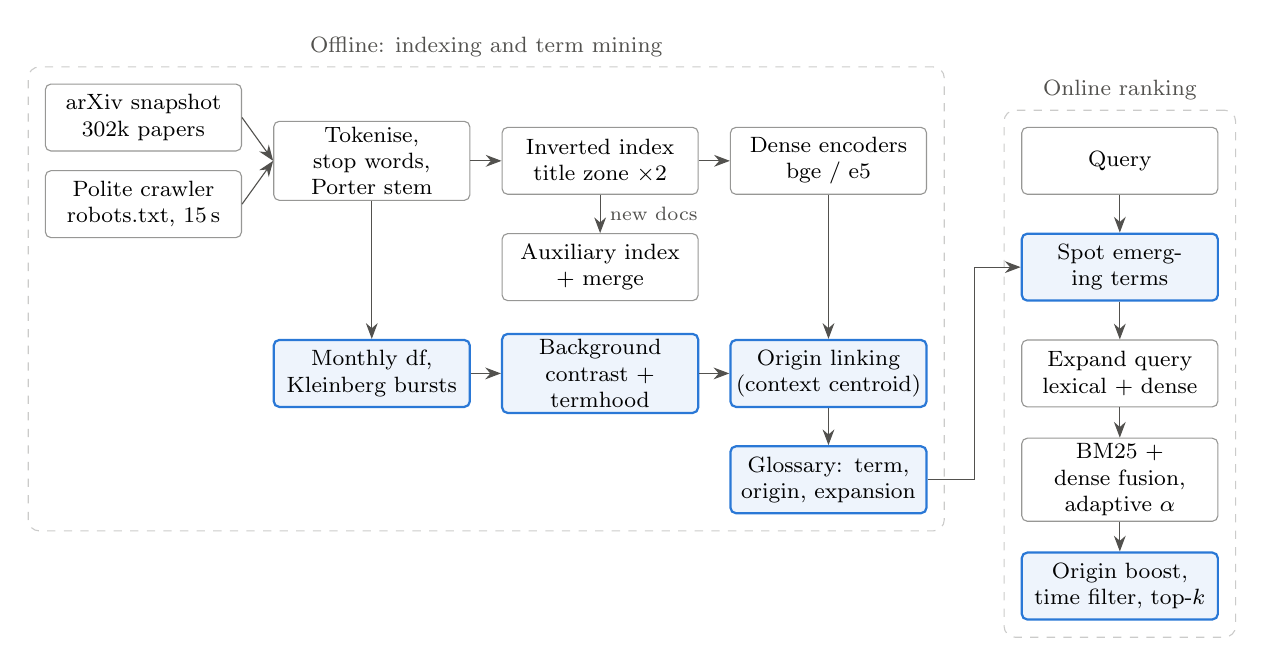
\begin{tikzpicture}[font=\footnotesize,
  box/.style={draw=mut!60,rounded corners=2pt,fill=white,align=center,text width=2.35cm,minimum height=0.85cm,inner sep=2pt},
  hot/.style={box,draw=acc,fill=acc!8,thick},
  arr/.style={-{Stealth[length=2mm]},mut}]
\node[box] (snap) at (0,0.55) {arXiv snapshot\\302k papers};
\node[box] (crawl) at (0,-0.55) {Polite crawler\\robots.txt, 15\,s};
\node[box] (tok) at (2.9,0) {Tokenise, stop words, Porter stem};
\node[box] (inv) at (5.8,0) {Inverted index\\title zone $\times2$};
\node[box] (enc) at (8.7,0) {Dense encoders\\bge / e5};
\node[box] (aux) at (5.8,-1.35) {Auxiliary index\\+ merge};
\node[hot] (burst) at (2.9,-2.7) {Monthly df,\\Kleinberg bursts};
\node[hot] (filt) at (5.8,-2.7) {Background contrast + termhood};
\node[hot] (link) at (8.7,-2.7) {Origin linking\\(context centroid)};
\node[hot] (gloss) at (8.7,-4.05) {Glossary: term, origin, expansion};
\node[box] (q) at (12.4,0) {Query};
\node[hot] (spot) at (12.4,-1.35) {Spot emerging terms};
\node[box] (exp) at (12.4,-2.7) {Expand query\\lexical + dense};
\node[box] (fuse) at (12.4,-4.05) {BM25 + dense fusion, adaptive $\alpha$};
\node[hot] (boost) at (12.4,-5.4) {Origin boost, time filter, top-$k$};
\draw[arr] (snap.east) -- (tok.west);
\draw[arr] (crawl.east) -- (tok.west);
\draw[arr] (tok) -- (inv);
\draw[arr] (inv) -- (enc);
\draw[arr] (inv) -- node[right,mut,font=\scriptsize]{new docs} (aux);
\draw[arr] (tok) -- (burst);
\draw[arr] (burst) -- (filt);
\draw[arr] (filt) -- (link);
\draw[arr] (enc) -- (link);
\draw[arr] (link) -- (gloss);
\draw[arr] (q) -- (spot);
\draw[arr] (spot) -- (exp);
\draw[arr] (exp) -- (fuse);
\draw[arr] (fuse) -- (boost);
\draw[arr] (gloss.east) -- (10.55,-4.05) |- (spot.west);
\begin{scope}[on background layer]
\node[draw=mut!30,dashed,rounded corners,fit=(snap)(crawl)(gloss)(enc),inner sep=6pt,label={[mut]above:Offline: indexing and term mining}] {};
\node[draw=mut!30,dashed,rounded corners,fit=(q)(boost),inner sep=6pt,label={[mut]above:Online ranking}] {};
\end{scope}
\end{tikzpicture}
\caption{Frontier pipeline. Blue boxes are the new emerging-term components.}
\label{fig:arch}
\end{figure*}

\section{Methodology}
\subsection{Indexing}
Titles and abstracts are lower-cased and split into alphanumeric tokens. Stop words
are removed and tokens are Porter-stemmed (with a cache). A title occurrence counts
twice, which gives a simple zone weighting. Postings are stored as a compressed
sparse row matrix (terms $\times$ documents) holding term frequencies; this is the
dictionary + postings structure with document ids in increasing order. Index
statistics are in Table~\ref{tab:index}. Storing the gaps between document ids with
variable-byte or $\gamma$ codes would shrink the postings about 3.5--4$\times$, and
the collection follows Zipf's law (Fig.~\ref{fig:zipf}).

\textbf{Dynamic indexing.} Papers crawled each day go into an auxiliary index that
shares the dictionary (new terms are appended). Queries score both indexes with
global statistics ($N$, df). Once the auxiliary index exceeds 5{,}000 documents it
is merged into the main index. A content-seen check (id and SHA-1 fingerprint of the
normalised text) skips duplicates.

\begin{table}[t]
\centering\small
\caption{Inverted index statistics.}
\label{tab:index}
\begin{tabular}{lrr}
\toprule
Statistic & arXiv & LitSearch \\
\midrule
Documents & 302,070 & 64,183 \\
Dictionary terms & 234,984 & 85,463 \\
Postings & 26,545,143 & 3,507,667 \\
Tokens (title x2) & 42,285,192 & 5,732,367 \\
Average document length & 139.98 & 89.31 \\
Postings, 32-bit ids (MB) & 101.26 & 13.38 \\
Postings, VB gaps (MB) & 28.84 & 4.0 \\
Postings, $\gamma$ gaps (MB) & 25.46 & 3.89 \\
Zipf slope & -1.691 & -1.633 \\
\bottomrule
\end{tabular}

\end{table}

\subsection{Retrieval models}
For query $q$ and document $d$ with term frequency $\mathrm{tf}_{t,d}$, document length
$|d|$ and average length $\overline{|d|}$:

\textbf{BM25}~\cite{robertson2009}:
\begin{equation}
s(q,d)=\sum_{t\in q} \mathrm{idf}_t\,\frac{\mathrm{tf}_{t,d}\,(k_1+1)}{\mathrm{tf}_{t,d}+k_1\big(1-b+b\frac{|d|}{\overline{|d|}}\big)},
\end{equation}
with $\mathrm{idf}_t=\log\big(1+\frac{N-\mathrm{df}_t+0.5}{\mathrm{df}_t+0.5}\big)$.
$k_1$ and $b$ are tuned on the dev split ($k_1=\CfgKone$, $b=\CfgB$).

\textbf{TF-IDF (SMART lnc.ltc)}: documents get $1+\log\mathrm{tf}$ weights with cosine
normalisation, queries get $(1+\log\mathrm{tf})\cdot\log(N/\mathrm{df})$, and the score is
their dot product.

\textbf{Query likelihood} with Dirichlet smoothing~\cite{zhai2001} ($\mu=1000$):
$s(q,d)=\sum_{t\in q}\log\frac{\mathrm{tf}_{t,d}+\mu P(t|C)}{|d|+\mu}$.

\textbf{Pseudo-relevance feedback.} We take the top 10 BM25 documents, add the 20
terms with the highest average normalised $\mathrm{tf}\cdot\mathrm{idf}$ to the query
with weight $0.5$ (Rocchio with $\gamma=0$), and re-score.

\textbf{Dense retrieval.} bge-small-en-v1.5~\cite{xiao2024} and
e5-small-v2~\cite{wang2022} (33M parameters each, both trained in 2022--23) embed
``title. abstract''. The score is the cosine similarity with the query embedding.

\textbf{Hybrid.} Each model returns its top 1{,}000 documents. Over the union
$P$, the scores are min-max normalised and combined:
\begin{equation}
s(d)=\alpha\,\hat s_{\text{BM25}}(d)+(1-\alpha)\,\hat s_{\text{dense}}(d).
\end{equation}

\textbf{Boolean retrieval} supports AND, OR, NOT, parentheses and quoted phrases, which are matched as conjunctions because the index stores no positions (parsed
with the shunting-yard algorithm, with postings intersected in order of increasing
length). \textbf{PageRank}~\cite{page1999} over the LitSearch citation graph
(345k edges) gives a static quality prior $g(d)$.

\subsection{Emerging-term detection}
\textbf{Candidates.} We take all 1--3-grams of titles and abstracts that contain no
stop word and are not pure numbers. For each month $m$ we count the papers that
contain the gram, $r_m$, out of $d_m$ papers that month.

\textbf{Growth and contrast.} A candidate needs (a) at least 30 papers overall and 20
in the last six months, (b) a recent rate at least 8 times its rate in the first 18
months, and (c) a recent rate at least 50 times its rate in the older
background corpus (64k LitSearch papers, 2017--2024). Condition (c) applies the
weirdness idea~\cite{ahmad1999} over time. Without it, the top ``emerging terms''
were \emph{every}, \emph{alone} and \emph{strongest}: a 2026 shift in how abstracts
are written, not new concepts.

\textbf{Kleinberg bursts.} For each surviving candidate we fit the two-state burst
automaton~\cite{kleinberg2002}. The base state emits at $p_0=\sum r_m/\sum d_m$ and the
burst state at $p_1=3p_0$. The emission cost of state $i$ in month $m$ is
\begin{equation}
c_i(m)=-\big[r_m\log p_i+(d_m-r_m)\log(1-p_i)\big],
\end{equation}
and entering the burst state costs $\gamma\ln n$ ($\gamma=1$, $n$ months). The
cheapest state sequence is found by Viterbi dynamic programming. A term is
\emph{emerging} if its last burst starts in July 2024 or later and its rate before
the burst is under a quarter of its rate during it. Terms are ranked by burst weight
$\sum_{m\in\text{burst}}(c_0(m)-c_1(m))$.

\textbf{Termhood.} We keep terms that contain capitals or digits after the first
character (GRPO, Qwen3-8B). We drop single lower-case words that are common in
general English (word frequency $\geq 2.5$ on the Zipf scale) and phrases with
adverbs. The remaining lower-case terms must appear in at least 5\% of the titles
that use them. Overlapping n-grams with similar counts are merged, keeping the
longer one (``model context protocol'' rather than ``context protocol''). We keep
the top \NGloss{}.

\subsection{Origin linking (term disambiguation)}
The earliest paper that ``introduces'' an acronym is often a different concept
altogether. MCP first appears in our corpus as a 2023 \emph{Mass-Conserving
Perceptron}, and DAPO and LLaDA have similar homonyms. We treat linking as entity
disambiguation. Let $c$ be the normalised mean bge embedding of up to 400 papers
that use the term during its burst. Candidates are early papers that define the term
(it is in the title, or in a sentence with ``we propose/introduce/present''). We link
to the \emph{earliest} candidate $d$ with $\cos(d,c)\geq\max_{d'}\cos(d',c)-0.065$.
The glossary stores, per term, the origin paper, a definition sentence and the ten
highest-weighted stems of the origin paper as expansion terms.

\subsection{Emerging-term-aware ranking}
Given query $q$, we spot glossary terms by matching n-grams (longest match first),
giving the set $E(q)$.
(1) \emph{Lexical expansion}: the BM25 query becomes
$q'=q+\beta\sum_{e\in E(q)}\sum_{w}\frac{x_{e,w}}{\max x}\,w$, using the expansion
weights $x$.
(2) \emph{Dense expansion}: the text ``$e$: title of the origin paper'' is appended
to the query before encoding.
(3) \emph{Adaptive fusion}: $\alpha$ becomes $\alpha_E$ when $E(q)\neq\emptyset$.
(4) \emph{Origin boost}: the origin papers are added to the pool and get $+\lambda$.
On LitSearch we optionally add $\mu\,g(d)$ from PageRank. The parameters
$(\alpha,\alpha_E,\beta,\lambda,k_1,b)$ are grid-searched on the dev split to
maximise nDCG@10. The selected values were $\alpha=\CfgAlpha$,
$\alpha_E=\CfgAlphaE$, $\beta=\CfgBeta$, $\lambda=\CfgLink$, $k_1=\CfgKone$ and
$b=\CfgB$. The origin boost (4) is applied only to \emph{named} terms (containing
capitals or digits after the first character), since generic concepts such as
``verifier'' have no single introducing paper. Size variants (Qwen3-4B) inherit the
origin of their model family (Qwen3), and a candidate whose title \emph{starts} with
the term (``Qwen3 Technical Report'', ``DAPO: \ldots'') is preferred.

\subsection{Fresh-2026 benchmark construction}
We sampled 420 papers from September--October 2026 with a primary category in
cs.CL, cs.IR, cs.LG or cs.AI, and fetched their arXiv HTML. robots.txt allows
\texttt{/html} and asks for a 15\,s crawl delay, which we respect. For each citation
in the body text we resolve the bibliography entry to a corpus paper, through an
arXiv identifier or an exact match of the normalised title. A sentence becomes a
query if it cites one or two corpus papers that are all resolvable and older than
the citing paper, and has 8--60 words without math, code or figure references. The
citation markers are removed. We keep at most four queries per paper. The
cited papers are the relevant documents. Retrieval is \emph{time-aware}: only papers
published before the citing paper may be returned, which simulates searching at that
date. Queries are split by citing paper into dev and test halves, so no paper
contributes to both. Each query is labelled by the age of its cited papers:
\emph{old} (before July 2024), \emph{new} (after July 2025) or \emph{mixed}. The
glossary is built only from papers before September 2026, so it never sees the
citing papers.

\subsection{Evaluation metrics}
For a query with relevant set $R$ and ranking $d_1,d_2,\dots$:
recall $R@k=|R\cap\{d_1..d_k\}|/|R|$; precision $P@k=|R\cap\{d_1..d_k\}|/k$;
$\mathrm{nDCG@10}=\frac{1}{Z}\sum_{i=1}^{10}\frac{[d_i\in R]}{\log_2(i+1)}$;
$\mathrm{MRR}=1/\text{rank of the first relevant}$;
$\mathrm{AP}=\frac{1}{|R|}\sum_{i:d_i\in R}P@i$, averaged as MAP. We also plot 11-point
interpolated precision--recall curves. Term detection is scored as a classification
with precision, recall, F1 and accuracy against manual labels. Significance uses
paired two-sided t-tests and Wilcoxon signed-rank tests over queries~\cite{smucker2007}.

\section{Experimentation and Results}
\subsection{Datasets}
\textbf{arXiv corpus.} The 27~October~2026 arXiv metadata snapshot, filtered to
papers listed in cs.CL, cs.LG, cs.AI or cs.IR and first submitted between January
2023 and October 2026: \NDocs{} titles and abstracts and \NTerms{} index terms.
\textbf{Fresh-2026.} We requested 201 sampled papers before arXiv began throttling
the crawler. \NCrawled{} had an HTML version, and \NPapers{} produced at least one
valid query, giving \NFresh{} queries: \NDev{} for tuning (dev) and \NTest{} for
testing. \NTermQ{} test queries contain an emerging term.
\textbf{LitSearch}~\cite{ajith2024}: 597 queries (inline-citation and author-written,
specific and broad) over \NLitDocs{} ACL/ICLR papers. We use the published titles and
abstracts and report recall@5 for specific and recall@20 for broad questions, as the
paper does.
\textbf{Term labels.} 230 terms were labelled as genuine new technical
terms or not: the top 60 detected terms, a random sample of 70 other detected terms,
60 rejected high-growth candidates, and a reference list of 40 well-known
2024--2026 terms. The origin links of \OriginNamed{} named artefacts (methods,
models, benchmarks, tools) were also checked.

\textbf{Setup.} All parameters are tuned on the Fresh-2026 dev split and then fixed;
LitSearch is never used for tuning. Everything runs on one laptop (Apple M4 Pro,
48\,GB). Mean latency per query over \NDocs{} papers is \LatBm{}\,ms for BM25 and
\LatFrontier{}\,ms for Frontier, including query encoding on the GPU
(Fig.~\ref{fig:lat}).

\subsection{Main results on Fresh-2026}
Table~\ref{tab:fresh} lists all systems on the test split. Frontier is best on every
metric: nDCG@10 \FrontierNdcg{}, against \HybridNdcg{} for the tuned hybrid,
\TfidfNdcg{} for TF-IDF, \BmNdcg{} for BM25 and \BgeNdcg{} for bge-small. The
improvement over the hybrid is significant ($p_t=\SigP$; better on \SigWins{}
queries, worse on \SigLosses{}). Fusion is the largest step among the baselines: it
adds 4 points over BM25 and 9 over bge-small, because lexical and dense retrievers
fail on different queries. The small 2023 embedders are weaker than BM25 on their
own on this domain, as BEIR~\cite{thakur2021} also found out of domain.
Table~\ref{tab:sig} gives all paired tests.

\begin{table}[t]
\centering\small\setlength{\tabcolsep}{4pt}
\caption{Fresh-2026 test split (\NTest{} queries, time-aware). $+E$ marks
emerging-term expansion. Best in bold.}
\label{tab:fresh}
\resizebox{\linewidth}{!}{\begin{tabular}{lrrrrrr}
\toprule
System & R@5 & R@20 & R@100 & nDCG@10 & MRR & MAP \\
\midrule
TF-IDF & 41.4 & 53.2 & 62.3 & 42.1 & 42.6 & 39.5 \\
QL-Dirichlet & 40.5 & 50.5 & 59.5 & 39.2 & 39.2 & 36.4 \\
BM25 & 42.4 & 50.9 & 59.5 & 40.9 & 41.2 & 38.2 \\
BM25{+}PRF & 42.1 & 50.7 & 58.8 & 39.4 & 39.3 & 36.4 \\
BM25{+}E & 43.1 & 51.4 & 60.0 & 41.4 & 41.7 & 38.7 \\
e5-small & 34.3 & 44.9 & 53.0 & 31.1 & 31.3 & 28.4 \\
e5-small{+}E & 34.7 & 45.4 & 55.6 & 32.0 & 32.4 & 29.2 \\
bge-small & 39.1 & 48.4 & 58.6 & 36.3 & 36.9 & 33.0 \\
bge-small{+}E & 39.1 & 49.5 & 59.3 & 36.7 & 37.4 & 33.6 \\
Hybrid & 46.3 & 57.4 & 69.4 & 45.0 & 46.1 & 42.9 \\
Hybrid{+}E & 47.7 & 57.9 & 69.9 & 45.8 & 46.4 & 43.4 \\
Frontier & \textbf{49.5} & \textbf{60.0} & \textbf{70.8} & \textbf{47.8} & \textbf{48.5} & \textbf{45.1} \\
\bottomrule
\end{tabular}
}
\end{table}

\begin{figure}[t]
\centering
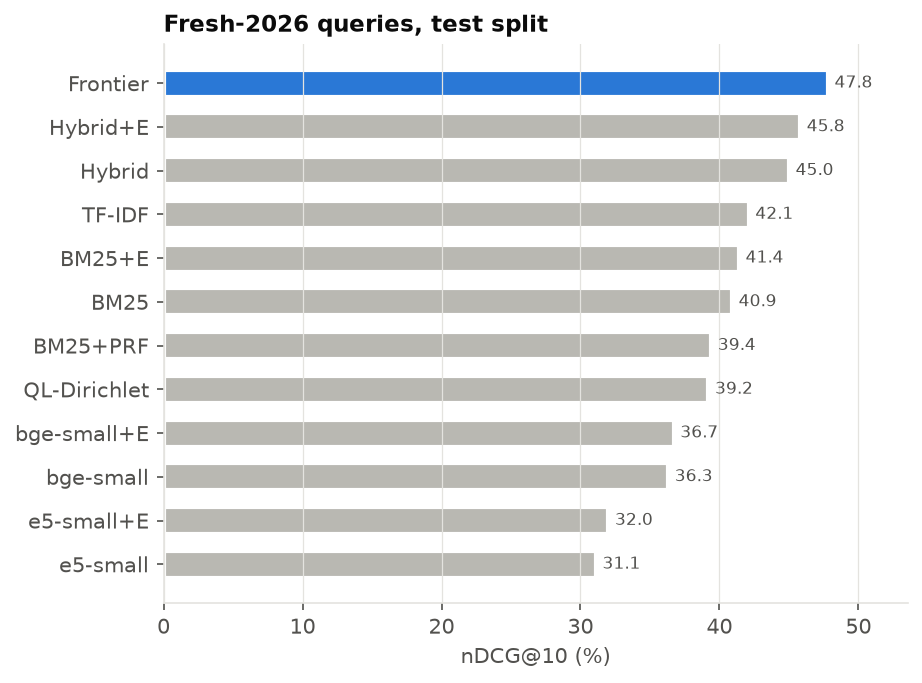
\includegraphics[width=\linewidth]{../results/figs/fresh_ndcg.png}
\caption{nDCG@10 on the Fresh-2026 test split.}
\label{fig:freshbar}
\end{figure}

\subsection{Effect of emerging terms}
Table~\ref{tab:hasterm} and Fig.~\ref{fig:hasterm} split the test queries by whether
they contain an emerging term.

\textbf{(1) All baselines struggle on new vocabulary.} BM25 drops from \NoTermBm{}
to \TermBm{} nDCG@10. Emerging terms are not rare tokens: GRPO appears in 1{,}800
papers and Qwen3 in hundreds, so they get a low IDF and match many papers that merely
\emph{use} the term. The cited paper, however, is usually the one that
\emph{introduced} it. The dense models also lose 10--18 points.

\textbf{(2) Expansion helps every retriever}: BM25 \TermBm{} $\rightarrow$
\TermBmE{}, bge-small \TermBge{} $\rightarrow$ \TermBgeE{}, e5-small \TermEfive{}
$\rightarrow$ \TermEfiveE{}, hybrid \TermHybrid{} $\rightarrow$ \TermHybridE{}. The
gains are consistent, but with \NTermQ{} queries none is significant on its own.

\textbf{(3) Origin linking gives the largest gain}: Frontier reaches \TermFrontier{}
on these queries, \textbf{+12.6 points over the hybrid} ($p_t=\TermSigP$, better on
\TermSigWins{} queries, worse on \TermSigLosses{}). Linking a named term to its
introducing paper is exactly what an inline citation needs.

\textbf{(4) No harm elsewhere}: on queries without emerging terms Frontier equals the
hybrid (\NoTermFrontier{} vs.\ \NoTermHybrid{}), because the layer only switches on
when a term is found.

\begin{table}[t]
\centering\small
\caption{nDCG@10 on test queries with and without an emerging term.}
\label{tab:hasterm}
\begin{tabular}{lrr}
\toprule
System & no emerging term & emerging term \\
\midrule
BM25 & 46.7 & 19.9 \\
bge-small & 38.4 & 28.6 \\
e5-small & 35.0 & 16.9 \\
Hybrid & \textbf{49.9} & 27.4 \\
Hybrid{+}E & \textbf{49.9} & 31.1 \\
Frontier & \textbf{49.9} & \textbf{40.0} \\
\bottomrule
\end{tabular}

\end{table}

\begin{figure}[t]
\centering
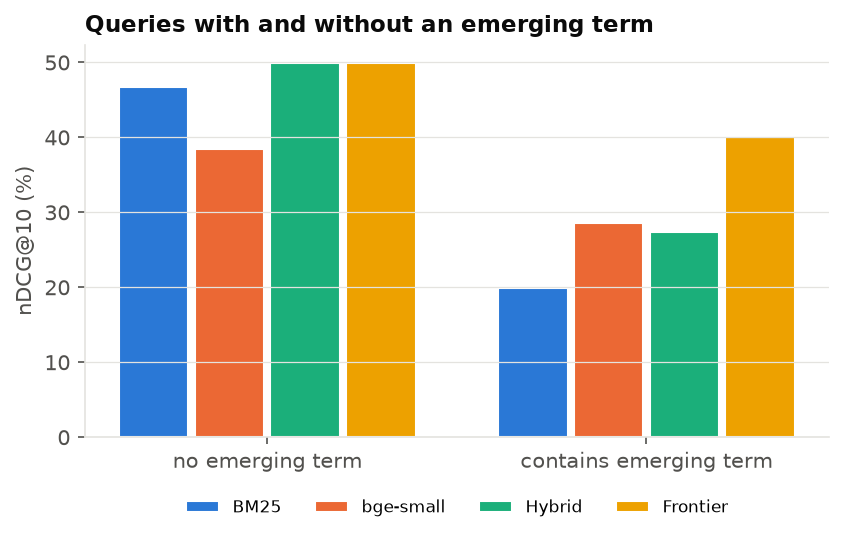
\includegraphics[width=\linewidth]{../results/figs/has_term.png}
\caption{nDCG@10 by query type: every baseline drops on new vocabulary; Frontier
recovers most of the gap.}
\label{fig:hasterm}
\end{figure}

\textbf{Age of the cited paper.} Table~\ref{tab:era} splits queries by when the cited
paper appeared. Every system finds queries about \emph{new} papers (after July 2025)
easier, because recent work is usually cited by a distinctive name. The gap between
BM25 and the 2023 dense model, however, is widest exactly there: \EraNewBm{} vs.\
\EraNewBge{} for new papers, against \EraOldBm{} vs.\ \EraOldBge{} for papers from
before July 2024. This fits the vocabulary drift that motivates our work. Frontier is
best in every age group.

\begin{table}[t]
\centering\small
\caption{nDCG@10 by publication date of the cited paper (test split).}
\label{tab:era}
\begin{tabular}{lrrr}
\toprule
System & before 2024-07 & mixed & after 2025-07 \\
\midrule
BM25 & 34.8 & 34.1 & 59.2 \\
bge-small & 29.8 & 32.7 & 50.4 \\
e5-small & 26.5 & 24.1 & 47.8 \\
Hybrid & 37.4 & 38.9 & 64.6 \\
Hybrid{+}E & 37.7 & 41.2 & 64.1 \\
Frontier & \textbf{40.4} & \textbf{42.7} & \textbf{65.4} \\
\bottomrule
\end{tabular}

\end{table}

\begin{table*}[t]
\centering\small
\caption{Paired significance tests on the Fresh-2026 test split. W/L = queries
where A is better / worse than B; $p_t$ paired t-test, $p_W$ Wilcoxon signed-rank.}
\label{tab:sig}
\begin{tabular}{llrrrrr}
\toprule
Comparison & Metric & Mean A & Mean B & W/L & $p_t$ & $p_W$ \\
\midrule
Frontier vs Hybrid & nDCG@10 & 47.8 & 45.0 & 14/3 & 0.013 & 0.010 \\
Frontier vs Hybrid & R@20 & 60.0 & 57.4 & 6/1 & 0.027 & 0.019 \\
Frontier vs BM25 & nDCG@10 & 47.8 & 40.9 & 43/19 & 2e-5 & 3e-5 \\
Frontier vs BM25 & R@20 & 60.0 & 50.9 & 24/3 & 2e-5 & 3e-5 \\
Frontier vs bge-small & nDCG@10 & 47.8 & 36.3 & 72/15 & 3e-8 & 3e-8 \\
Frontier vs bge-small & R@20 & 60.0 & 48.4 & 39/8 & 4e-6 & 1e-5 \\
Hybrid{+}E vs Hybrid & nDCG@10 & 45.9 & 45.0 & 9/3 & 0.177 & 0.147 \\
Hybrid{+}E vs Hybrid & R@20 & 57.9 & 57.4 & 2/2 & 0.528 & 0.458 \\
BM25{+}E vs BM25 & nDCG@10 & 41.4 & 40.9 & 5/1 & 0.144 & 0.075 \\
BM25{+}E vs BM25 & R@20 & 51.4 & 50.9 & 1/0 & 0.318 & 0.317 \\
bge-small{+}E vs bge-small & nDCG@10 & 36.7 & 36.3 & 8/7 & 0.616 & 0.570 \\
bge-small{+}E vs bge-small & R@20 & 49.5 & 48.4 & 5/3 & 0.298 & 0.248 \\
Hybrid vs BM25 & nDCG@10 & 45.0 & 40.9 & 35/19 & 0.001 & 0.002 \\
Hybrid vs BM25 & R@20 & 57.4 & 50.9 & 20/4 & 9e-4 & 0.001 \\
\bottomrule
\end{tabular}

\end{table*}

\subsection{Comparison with a published paper: LitSearch}
Table~\ref{tab:lit} compares our systems with the results published in
LitSearch~\cite{ajith2024}, using the same queries, corpus and metrics. Our BM25
(stemming, title zone, $k_1,b$ tuned on Fresh-2026) reaches \LitBm{} recall@5 on
specific questions, against 50.0 published. Our hybrid of BM25 and the 33M-parameter
bge-small reaches \LitHybrid{} (broad recall@20 \LitBroadHybrid{}). This beats the
published E5-large-v2 (56.2/55.4) and Instructor-XL (52.3/56.5), and narrows the gap
to GritLM-7B (74.8/70.8), a model about 200 times larger.
LitSearch's papers predate our emerging terms: only \LitTermQ{} of its 597 queries
contain one, and no origin links exist in that corpus. Frontier therefore behaves
exactly like the hybrid there (\LitFrontier{}), which shows the new layer is safe on
older literature. The PageRank prior leaves recall@5 unchanged but gives a small,
significant nDCG@10 gain (\LitFrontierNdcg{} $\rightarrow$ \LitPrNdcg{},
$p_t=\LitPrP$). Citation authority helps break ties between candidates.

\begin{table*}[t]
\centering\small
\caption{LitSearch: our systems (top) against the published results of
Ajith et al.~\cite{ajith2024} (bottom). Recall@5 for specific and recall@20 for broad
questions, titles and abstracts only.}
\label{tab:lit}
\begin{tabular}{lrrrrrr}
\toprule
System & \multicolumn{2}{c}{Inline-citation} & \multicolumn{2}{c}{Author-written} & \multicolumn{2}{c}{Average} \\
 & Spec.\ R@5 & Broad R@20 & Spec.\ R@5 & Broad R@20 & Spec.\ R@5 & Broad R@20 \\
\midrule
TF-IDF & 43.5 & 43.3 & 60.2 & 51.4 & 51.5 & 45.1 \\
QL-Dirichlet & 43.7 & 41.4 & 61.1 & 60.0 & 52.0 & 45.6 \\
BM25 & 46.5 & 44.6 & 65.9 & 57.1 & 55.8 & 47.5 \\
BM25{+}PRF & 41.8 & 45.9 & 63.0 & 57.1 & 51.9 & 48.4 \\
e5-small & 43.7 & 38.9 & 53.1 & 54.3 & 48.2 & 42.4 \\
bge-small & 51.9 & 59.4 & 55.5 & 57.1 & 53.6 & 58.9 \\
Hybrid & 55.6 & 58.3 & 73.5 & 68.6 & 64.1 & 60.6 \\
Frontier & 55.6 & 58.3 & 73.5 & 68.6 & 64.1 & 60.6 \\
Frontier{+}PageRank & 56.5 & 58.3 & 72.5 & 65.7 & 64.1 & 60.0 \\
\midrule
BM25 \cite{ajith2024} & 38.5 & 37.4 & 62.6 & 48.6 & 50.0 & 39.9 \\
GTR-T5-large \cite{ajith2024} & 38.5 & 45.7 & 40.8 & 37.1 & 39.6 & 43.8 \\
Instructor-XL \cite{ajith2024} & 48.9 & 56.3 & 55.9 & 57.1 & 52.3 & 56.5 \\
E5-large-v2 \cite{ajith2024} & 50.4 & 55.8 & 62.6 & 54.3 & 56.2 & 55.4 \\
GritLM-7B \cite{ajith2024} & 67.7 & 69.7 & 82.5 & 74.3 & 74.8 & 70.8 \\
\bottomrule
\end{tabular}

\end{table*}

\begin{figure}[t]
\centering
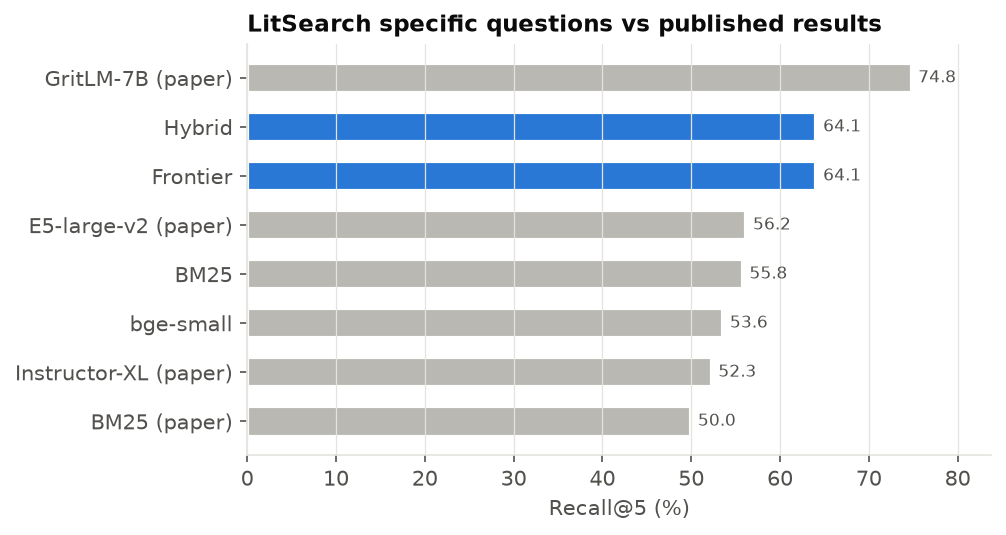
\includegraphics[width=\linewidth]{../results/figs/litsearch.png}
\caption{LitSearch specific questions: ours (blue) vs.\ published retrievers.}
\label{fig:lit}
\end{figure}

\subsection{Emerging-term detection and linking}
Table~\ref{tab:terms} scores term detection as a classification against the labels.
Precision is high among the top-ranked terms (\TopP{}) and lower in the long tail
(\RandP{} on a random sample of the rest). The detector recovers \RefR{} of the
reference terms and correctly rejects \RejAcc{} of the high-growth generic
candidates. The missed reference terms are mostly older ones whose burst began before
July 2024, such as \emph{test-time scaling} and \emph{LLM-as-a-judge}.
Origin linking is correct for \OriginCorrect{} of the \OriginNamed{} named
artefacts, i.e.\ \OriginAccOn{}\% of those whose introducing paper is on arXiv.
Examples: GRPO $\rightarrow$ DeepSeekMath, Qwen3-4B $\rightarrow$ Qwen3 Technical
Report, DAPO, GSPO, GEPA, DeepSeek-R1/V3, SWE-bench, BrowseComp, HarmBench, SGLang
and FineWeb-Edu. Product names announced outside arXiv (GPT-5.x, Claude Code, MCP)
are linked to an early paper about them instead. Context-based disambiguation is
essential here. Without it, MCP was linked to a 2023 \emph{Mass-Conserving
Perceptron}, DAPO to an unrelated \emph{Dual Approximation Policy Optimization}, and
LLaDA to a driving paper. Fig.~\ref{fig:bursts} shows detected bursts.

\begin{table}[t]
\centering\small\setlength{\tabcolsep}{4pt}
\caption{Emerging-term detection against manual labels.}
\label{tab:terms}
\begin{tabular}{lrrrrr}
\toprule
Set & $n$ & P & R & F1 & Acc. \\
\midrule
Top-60 detected & 60 & 0.61 & -- & -- & -- \\
Random detected & 70 & 0.22 & -- & -- & -- \\
Reference list & 40 & -- & 0.65 & -- & -- \\
Rejected & 60 & -- & -- & -- & 0.98 \\
Combined & 169 & 0.43 & 0.71 & 0.54 & 0.59 \\
\bottomrule
\end{tabular}

\end{table}

\begin{figure}[t]
\centering
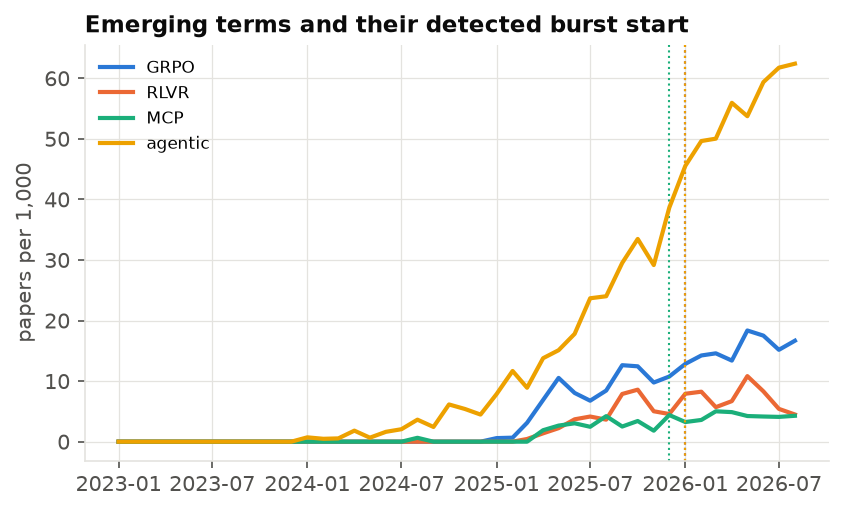
\includegraphics[width=\linewidth]{../results/figs/bursts.png}
\caption{Monthly rate of four emerging terms; dotted lines mark the start of the
latest burst found by Kleinberg's automaton.}
\label{fig:bursts}
\end{figure}

\begin{figure}[t]
\centering
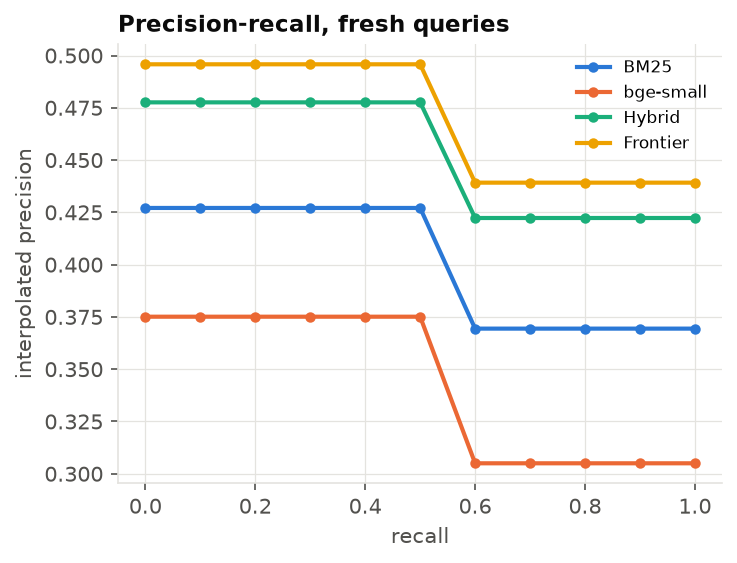
\includegraphics[width=0.49\linewidth]{../results/figs/pr_fresh.png}
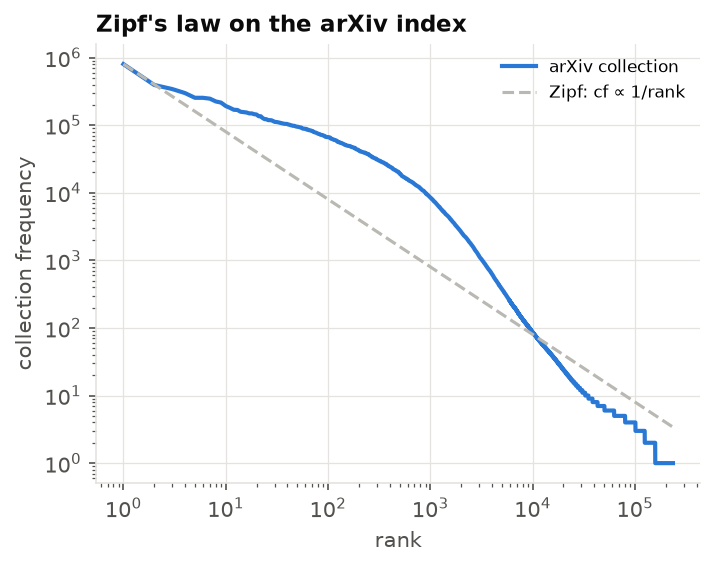
\includegraphics[width=0.49\linewidth]{../results/figs/zipf.png}
\caption{Left: interpolated precision--recall on Fresh-2026. Right: Zipf's law on
the arXiv index.}
\label{fig:zipf}
\end{figure}

\begin{figure}[t]
\centering
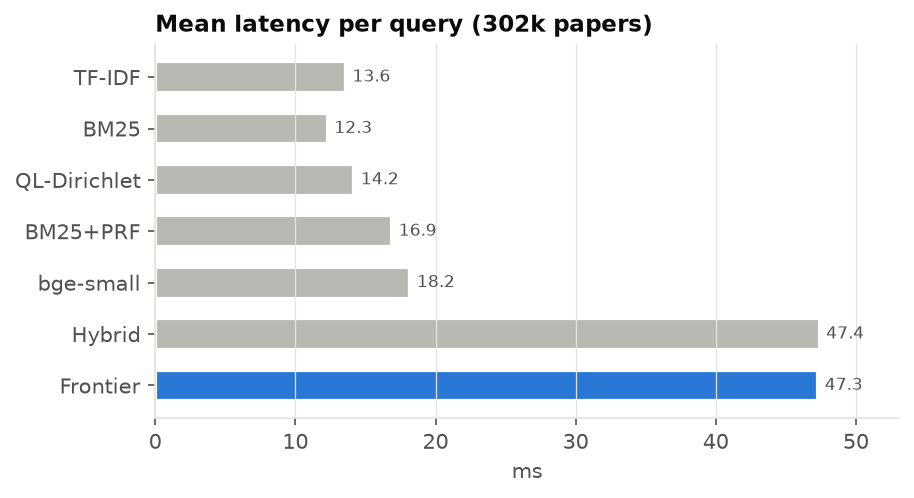
\includegraphics[width=0.9\linewidth]{../results/figs/latency.png}
\caption{Mean latency per query over \NDocs{} papers.}
\label{fig:lat}
\end{figure}

\subsection{Discussion}
Three lessons stand out. First, classic IR does most of the work. A tuned BM25 is a
strong baseline, and a simple min-max fusion with a small embedder beats much larger
dense models on LitSearch. Second, new vocabulary is a real weakness of \emph{both}
retriever families, but for different reasons. Lexical matching cannot tell which of
the many papers using a popular new term is meant. Dense models trained before the
term existed do not know what it means. Third, the most effective fix is not
richer matching but \emph{knowledge}: knowing which paper introduced a term. Tuning
on the dev split chose a strong origin boost ($\lambda=\CfgLink$) with light
expansion ($\beta=\CfgBeta$). It kept the same fusion weight with or without an
emerging term ($\alpha_E=\alpha=\CfgAlpha$), so the adaptive-fusion component turned
out to be unnecessary once expansion and linking were in place. The gains cost
nothing at query time: Frontier's latency equals the hybrid's (\LatHybrid{}\,ms).

\section{Conclusions and Limitations}
We built Frontier, a complete search engine for the latest AI research. Detecting
emerging terms from corpus statistics, and linking them to the papers that
introduced them, improves retrieval significantly. It adds +12.6 nDCG@10 on queries
with new vocabulary and +2.8 overall over a tuned hybrid, without retraining any
model or calling an LLM at query time. Our hybrid baseline also beats several much
larger published retrievers on LitSearch.

\textbf{Limitations.}
(1) Fresh-2026 is built automatically: a citation sentence is an imperfect query, an
author may cite one of several valid papers, and unresolved citations are dropped.
With \NTest{} test queries (\NTermQ{} with emerging terms), small differences are not
significant.
(2) The title-prefix and model-family rules for origin linking were added after
inspecting linking errors on Fresh-2026 queries from both splits. The test-split
gain of the origin boost may therefore be slightly optimistic.
(3) Term detection is noisy in the long tail (precision \RandP{}). The labels
come from the project itself, not from independent annotators.
(4) Origins cannot be found for terms introduced outside arXiv (blogs, product
launches).
(5) We use small 2023 embedders because of laptop compute. Newer models (e.g.\
Qwen3-Embedding) would raise all dense numbers, but their own training cutoff moves
the vocabulary gap rather than closing it.
(6) We index titles and abstracts only. arXiv HTML crawling at the required 15\,s
delay, plus throttling, limited Fresh-2026 to \NPapers{} citing papers.
\textbf{Future work}: extracting definitions for glossary entries without an LLM,
term-aware document expansion at index time, and a continuously refreshed benchmark.


\begin{thebibliography}{99}\small\itemsep0pt
\bibitem{ahmad1999} Ahmad, K., Gillam, L. and Tostevin, L., 1999, November. University of Surrey participation in TREC8: Weirdness indexing for logical document extrapolation and retrieval (WILDER). In Proceedings of the Eighth Text REtrieval Conference (TREC-8). NIST.
\bibitem{ajith2024} Ajith, A., Xia, M., Chevalier, A., Goyal, T., Chen, D. and Gao, T., 2024, November. LitSearch: A retrieval benchmark for scientific literature search. In Proceedings of the 2024 Conference on Empirical Methods in Natural Language Processing (pp. 15068--15083).
\bibitem{cohan2020} Cohan, A., Feldman, S., Beltagy, I., Downey, D. and Weld, D.S., 2020, July. SPECTER: Document-level representation learning using citation-informed transformers. In Proceedings of the 58th Annual Meeting of the Association for Computational Linguistics (pp. 2270--2282).
\bibitem{cormack2009} Cormack, G.V., Clarke, C.L. and Buettcher, S., 2009, July. Reciprocal rank fusion outperforms Condorcet and individual rank learning methods. In Proceedings of the 32nd International ACM SIGIR Conference on Research and Development in Information Retrieval (pp. 758--759).
\bibitem{he2025} He, Y., Huang, G., Feng, P., Lin, Y., Zhang, Y., Li, H. and E, W., 2025, July. PaSa: An LLM agent for comprehensive academic paper search. In Proceedings of the 63rd Annual Meeting of the Association for Computational Linguistics (pp. 11663--11679).
\bibitem{he2010} He, Q., Pei, J., Kifer, D., Mitra, P. and Giles, L., 2010, April. Context-aware citation recommendation. In Proceedings of the 19th International Conference on World Wide Web (pp. 421--430).
\bibitem{hu2026} Hu, T., Zhao, Y., Zhang, C., Cohan, A. and Zhao, C., 2026, February. SAGE: Benchmarking and improving retrieval for deep research agents. arXiv preprint arXiv:2602.05975.
\bibitem{kleinberg2002} Kleinberg, J., 2002, July. Bursty and hierarchical structure in streams. In Proceedings of the 8th ACM SIGKDD International Conference on Knowledge Discovery and Data Mining (pp. 91--101).
\bibitem{lazaridou2021} Lazaridou, A., Kuncoro, A., Gribovskaya, E., Agrawal, D., Liska, A., Terzi, T., Gimenez, M., de Masson d'Autume, C., Kocisky, T., Ruder, S., Yogatama, D., Cao, K., Young, S. and Blunsom, P., 2021, December. Mind the gap: Assessing temporal generalization in neural language models. In Advances in Neural Information Processing Systems 34 (pp. 29348--29363).
\bibitem{longeval2026} Wu, H. and Yang, Y., 2026, September. Submitted and diagnostic analysis of full-text temporal retrieval for LongEval-Sci. In Working Notes of CLEF 2026, CEUR Workshop Proceedings, Vol. 4283 (arXiv:2607.04088).
\bibitem{manning2008} Manning, C.D., Raghavan, P. and Sch\"utze, H., 2008. Introduction to Information Retrieval. Cambridge University Press.
\bibitem{mei2005} Mei, Q. and Zhai, C., 2005, August. Discovering evolutionary theme patterns from text: an exploration of temporal text mining. In Proceedings of the 11th ACM SIGKDD International Conference on Knowledge Discovery in Data Mining (pp. 198--207).
\bibitem{page1999} Page, L., Brin, S., Motwani, R. and Winograd, T., 1999. The PageRank citation ranking: Bringing order to the web. Technical report, Stanford InfoLab.
\bibitem{robertson2009} Robertson, S. and Zaragoza, H., 2009. The probabilistic relevance framework: BM25 and beyond. Foundations and Trends in Information Retrieval, 3(4), pp.333--389.
\bibitem{shi2025} Shi, X., Li, Y., Kou, Q., Yu, L., Xie, J. and Zhou, H., 2025, July. SPAR: Scholar paper retrieval with LLM-based agents for enhanced academic search. arXiv preprint arXiv:2507.15245.
\bibitem{smucker2007} Smucker, M.D., Allan, J. and Carterette, B., 2007, November. A comparison of statistical significance tests for information retrieval evaluation. In Proceedings of the 16th ACM Conference on Information and Knowledge Management (pp. 623--632).
\bibitem{thakur2021} Thakur, N., Reimers, N., R\"uckl\'e, A., Srivastava, A. and Gurevych, I., 2021, December. BEIR: A heterogeneous benchmark for zero-shot evaluation of information retrieval models. In Proceedings of the Neural Information Processing Systems Track on Datasets and Benchmarks.
\bibitem{wang2022} Wang, L., Yang, N., Huang, X., Jiao, B., Yang, L., Jiang, D., Majumder, R. and Wei, F., 2022, December. Text embeddings by weakly-supervised contrastive pre-training. arXiv preprint arXiv:2212.03533.
\bibitem{xiao2024} Xiao, S., Liu, Z., Zhang, P., Muennighoff, N., Lian, D. and Nie, J.Y., 2024, July. C-Pack: Packed resources for general Chinese embeddings. In Proceedings of the 47th International ACM SIGIR Conference on Research and Development in Information Retrieval (pp. 641--649).
\bibitem{zhai2001} Zhai, C. and Lafferty, J., 2001, September. A study of smoothing methods for language models applied to ad hoc information retrieval. In Proceedings of the 24th Annual International ACM SIGIR Conference on Research and Development in Information Retrieval (pp. 334--342).
\end{thebibliography}

\end{document}
